\documentclass[11pt]{beamer}
\usepackage[utf8]{inputenc}
\usepackage[frenchb]{babel}
\usepackage{graphicx}
\usepackage{textpos}
%\usepackage{movie15}
\usepackage{multimedia}
%\usepackage{media9}
%\usepackage{hyperref}
%\usepackage{url}

\usetheme{Berlin}%Boadilla
\usecolortheme{beaver}

\makeatletter
%\beamer@theme@subsectionfalse
\makeatother

\title{SIGVerse interaction trough Robot Operating System}
\author{Geneviève CIRERA}\institute{Polytech'Nice-Sophia}
%\subtitle{Soutenance intermédiaire d'apprentissage}
\date{\oldstylenums{\today}}

\begin{document}

\begin{frame}
\titlepage
\end{frame}

% --------- Sommaire -----------
%\begin{frame}{Plan}
%  \tableofcontents[sections={1}]
%  \tableofcontents[sections={2}]
%  \tableofcontents[sections={3}]
%\end{frame}

%\AtBeginSection[]{
%  \begin{frame}{Sommaire}
%  \small \tableofcontents[currentsection, hideothersubsections]
%  \end{frame} 
%}
% ------------------------------

% ----- Presentacion ------
\section{Introduction}

\subsection*{}
%\subsection{En bref}

%\movie{
\includegraphics[width=.65\textwidth]{images/SingleCleanUpDemo2014.png}}{videos/CleanUpReferee.mp4}
%\url{videos/CleanUpReferee.mp4}

\begin{frame}{RoboCup}		
	RoboCup competition, how to participate
	\begin{columns}[t]
		\begin{column}[T]{.5\textwidth}
			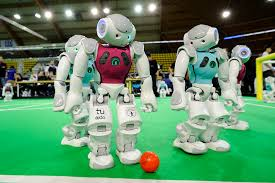
\includegraphics[width=1\textwidth]{images/robocupFoot.jpg}
		\end{column}
		\begin{column}[T]{.5\textwidth}
			\includegraphics[width=0.7\textwidth]{images/robocupHome.jpg}	
		\end{column}
	\end{columns}
\end{frame}

\begin{frame}{SIGVerse}		
\begin{columns}[t]
	\begin{column}[T]{.6\textwidth}
		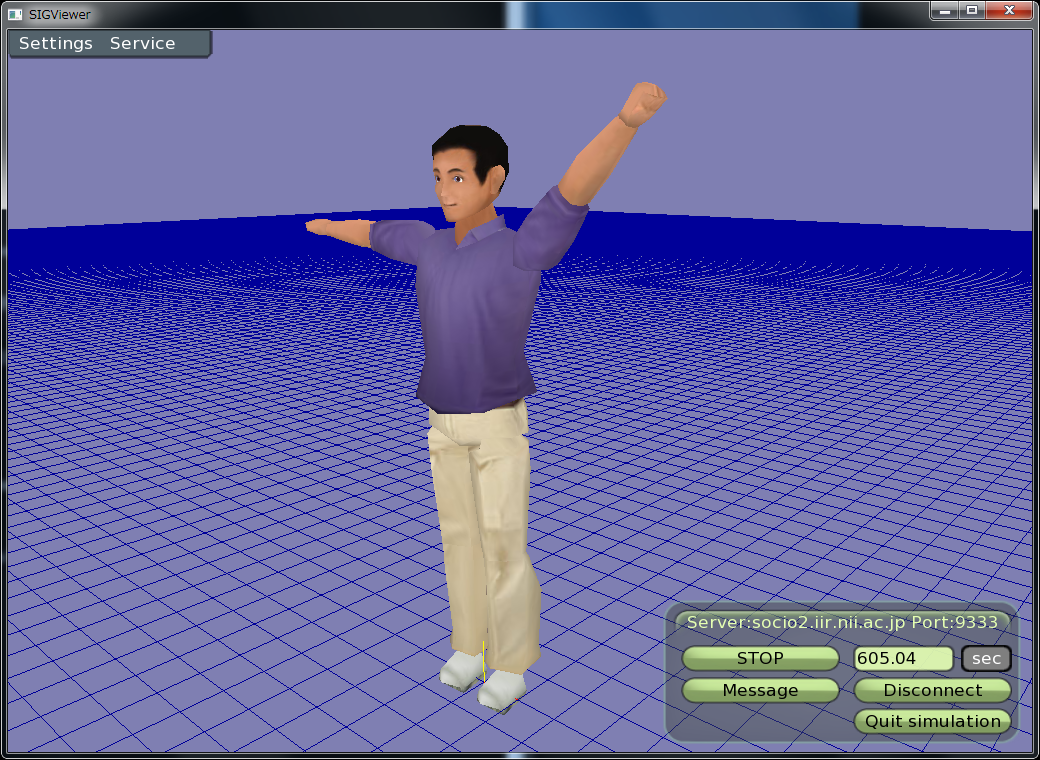
\includegraphics[width=1\textwidth]{images/manViewer.png}
	\end{column}
	\begin{column}[T]{.4\textwidth}
		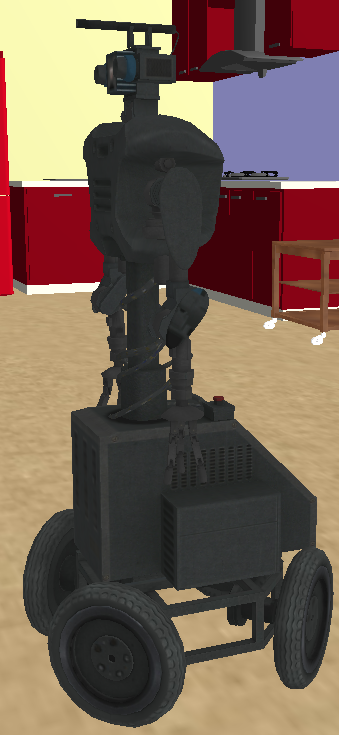
\includegraphics[width=0.6\textwidth]{images/robot_000_sigverse.png}
	\end{column}
\end{columns}
\end{frame}

\begin{frame}{Goal}
	\begin{itemize}
		\item C++
		\item Dynamique SIGVerse
		\item Japanese documentation
		\item Problem of SIGVerse (no restart without relaunch simulation)
		\item Robotic world : Robot Operating System
	\end{itemize}
\end{frame}

\begin{frame}{Goal}
	\begin{center}
		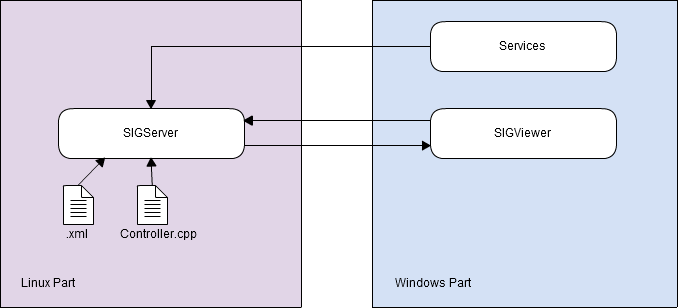
\includegraphics[width=0.65\textwidth]{images/SIGVerseSimple.png}\\
		\vspace{0.3cm}
		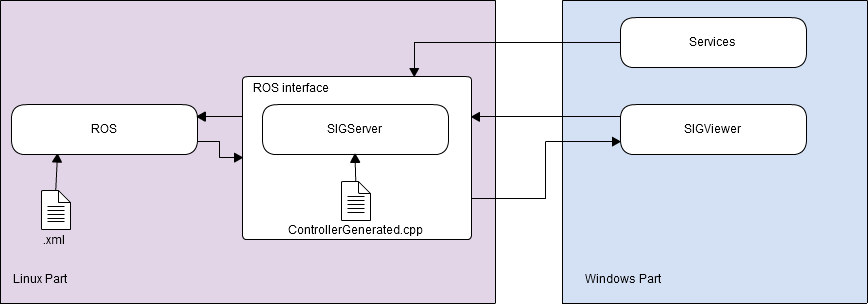
\includegraphics[width=0.7\textwidth]{images/SIGVerseROS.png}	
	\end{center}
\end{frame}

\section{sig\_ros}
\subsection*{}
\begin{frame}{Robot Operating System}
	\begin{center}
		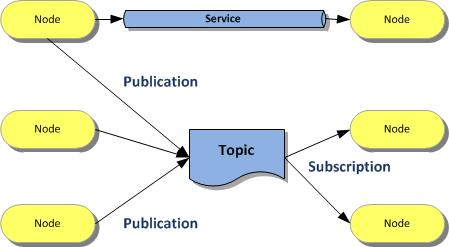
\includegraphics[width=0.8\textwidth]{images/Concepts-de-base-ROS.jpg}
	\end{center}
\end{frame}

\begin{frame}{Generalities}
	\begin{center}
		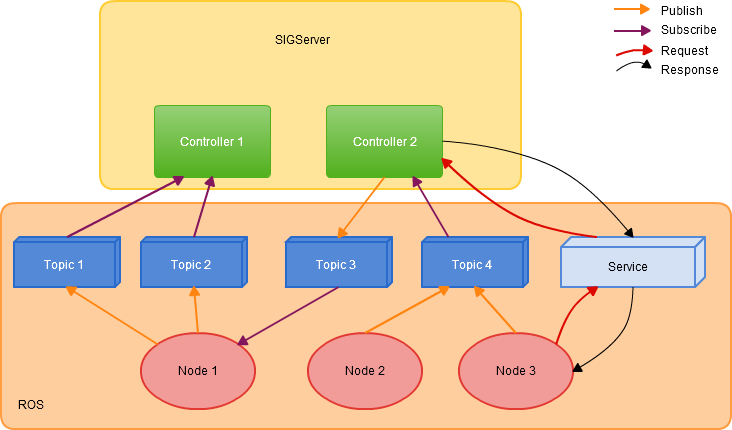
\includegraphics[width=0.8\textwidth]{images/sig_ros_general.png}
	\end{center}
\end{frame}

\begin{frame}{Package}
	\begin{center}
		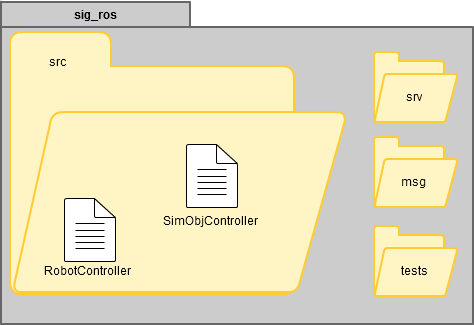
\includegraphics[width=0.7\textwidth]{images/package_sig_ros.png}
	\end{center}
\end{frame}

\begin{frame}{Use}
	\begin{center}
		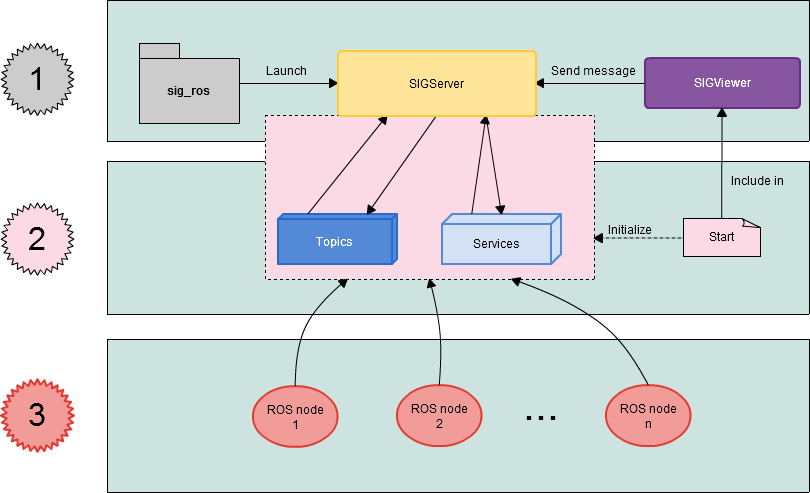
\includegraphics[width=0.8\textwidth]{images/usage.png}
	\end{center}
\end{frame}

\section{More functionnalities}
\subsection*{}
\begin{frame}{Inverse kinematics}
	\begin{center}
		%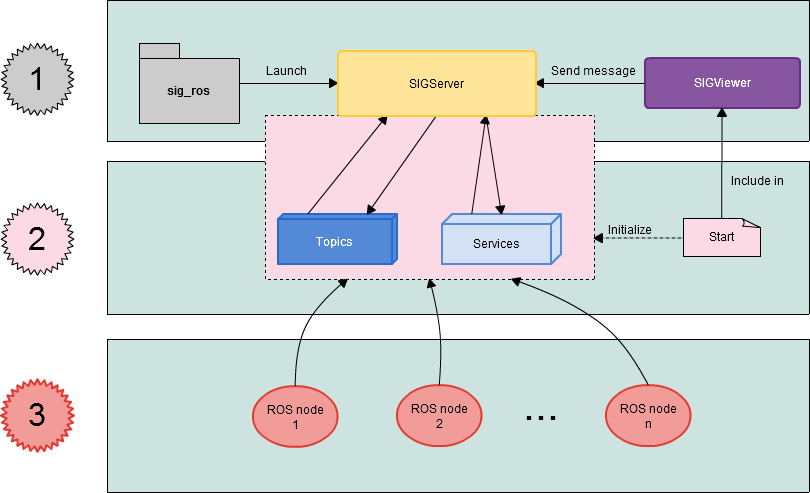
\includegraphics[width=0.8\textwidth]{images/usage.png}
	\end{center}
\end{frame}

\section{Conclusion}
\subsection*{}
\begin{frame}{Result}
%Vidéo
\end{frame}

\begin{frame}{To go further}
\end{frame}

\begin{frame}{Skills}
\end{frame}

\end{document}